\begin{definition}[Category~\cite{pierce1991basic,barr1990category}]
    \label{def:cat}
    A \textbf{category} is an unlabeled graph \( C \) together with a total function \( u : C_0 \to C_1 \) and a partial function \( \star: C_1 \times C_1 \to C_1 \) such that 
        (i) for all edges \( f:X \to Y \) and \( g:Y \to Z \), the edge \( f \star g :X \to Z \) is defined; 
        (ii) for every node \( X \), \( u(X) \) is an edge from \( X \) to \( X \);
        (iii) for every \( f:X \to Y \), we have \(u(X) \star f = f = f \star u(Y)\);
        (iv) for all edges \( f \), \( g \) and \(h\), we have \( (f \star g) \star h = f \star (g \star h) \) whenever either side is defined.
    Edges are called \textbf{morphisms}. The function $\star$ is called \textbf{composition}. For all \( X \in C_0 \), the edge \( u(X) \) is denoted \( \operatorname{id}_X \) and is called the \textbf{identity} of the object \( X \).
    % \( C \) is called the \textbf{underlying graph} of the category \( \mathcal{C} \).
\end{definition} 

% cat notation * 
\begin{notation}
    The composition of morphisms \( f : X \to Y \) and \( g : Y \to Z \) is written in diagrammatic order as \( f \star g \), rather than in functional order \( g \circ f \). 
    % The advantage is that, when reading from left to right, the morphisms appear in the same order as in the corresponding diagram, making the notation more intuitive for visual reasoning.
\end{notation}  

\begin{definition}[Monomorphism~\cite{pierce1991basic,barr1990category}]
    \label{def:cat:homo}
    A morphism \( f : X \to Y \) is \textbf{monic} (or a \textbf{monomorphism}) if for all morphisms \( g \) and \( h \), if \( g \star f = h \star f \), then \( g = h \). A monomorphism is denoted by \( f : X \rightarrowtail Y \). The set of all monomorphisms from graph \( X \) to graph \( Y \) is denoted by \( \operatorname{Mono}(X, Y) \).
\end{definition} 
\begin{example}
     Finite edge-labeled directed multigraphs and their homomorphisms form a category, hereafter denoted \textbf{Graph}. Its objects are labeled graphs, its morphisms are graph homomorphisms, and the monomorphisms are injective homomorphisms.
\end{example}
\begin{definition}[Category of Rewriting Systems]
    Rewriting systems and homomorphisms between them form a category, denoted $\mathcal{RS}$.   
  \end{definition}
In category theory, a ordered pair \((\alpha : A \to B,\, \beta : A \to C)\) of morphisms with a common domain is called a \textbf{span} \cite{lowe2010graph}, denoted by
\(
B \overset{\alpha}{\leftarrow} A \overset{\beta}{\rightarrow} C.
\)
Likewise, an ordered pair \((\beta' : B \to D,\, \alpha' : C \to D)\) of morphisms with a common codomain is called a \textbf{cospan}, denoted by
\(
B \overset{\beta'}{\rightarrow} D \overset{\alpha'}{\leftarrow} C.
\)

\begin{definition}[Diagram \cite{barr1990category}]
    \label{def:cat:diagram}
    Let \( G \) be an unlabeled graph. A \textbf{diagram} (in \( \mathcal{C} \) of shape \( G \)) is a homomorphism of unlabeled graphs $ h : G \to C $ where \( C \) is the underlying unlabeled graph of the category \( \mathcal{C} \). A diagram is \textbf{commutative} if, for all nodes \( u \), \( v \), and any two paths from \( u \) to \( v \) in the unlabeled graph \( G \):

    \begin{center}
    \resizebox{12cm}{!}{
        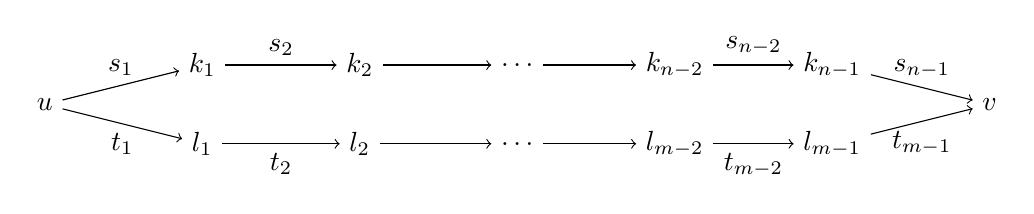
\begin{tikzpicture}
        \node (u) at (0,0) {\( u \)};
        \node (k1) at (2,0.5) {\( k_1 \)};
        \node (k2) at (4,0.5) {\( k_2 \)};
        \node (ketc) at (6,0.5) {\( \dots \)};
        \node (knm2) at (8,0.5) {\( k_{n-2} \)};
        \node (knm1) at (10,0.5) {\( k_{n-1} \)};
        \node (v) at (12,0) {\( v \)};
        \node (l1) at (2,-0.5) {\( l_1 \)};
        \node (l2) at (4,-0.5) {\( l_2 \)};
        \node (letc) at (6,-0.5) {\( \dots \)};
        \node (lnm2) at (8,-0.5) {\( l_{m-2} \)};
        \node (lnm1) at (10,-0.5) {\( l_{m-1} \)};
        \draw[->] (u) -- (k1) node [midway,above] {\( s_1 \)};
        \draw[->] (k1) -- (k2) node [midway,above] {\( s_2 \)};
        \draw[->] (k2) -- (ketc);
        \draw[->] (ketc) -- (knm2); 
        \draw[->] (knm2) -- (knm1) node[midway,above] {\( s_{n-2} \)}; 
        \draw[->] (knm1) -- (v) node[midway,above] {\( s_{n-1} \)}; 
        \draw[->] (u) -- (l1) node[midway,below] {\( t_1 \)};
        \draw[->] (l1) -- (l2) node[midway,below] {\( t_2 \)};
        \draw[->] (l2) -- (letc);
        \draw[->] (letc) -- (lnm2); 
        \draw[->] (lnm2) -- (lnm1) node[midway,below] {\( t_{m-2} \)}; 
        \draw[->] (lnm1) -- (v) node[midway,below] {\( t_{m-1} \)}; 
        \end{tikzpicture}
    }
    \end{center}
    \noindent
    the equality \( h(s_1) \star h(s_2) \star \dots  \star h(s_{n-1}) = h(t_1) \star h(t_2) \star \dots  \star h(t_{m-1}) \) holds.
\end{definition}

\begin{definition}[Pushout \cite{barr1990category}]
    \label{def:cat:po}
    \ \newline
\noindent
\begin{minipage}{0.7\textwidth}  
    A \textbf{pushout} of a span \( B \overset{\alpha}{\leftarrow} A \overset{\beta}{\rightarrow} C \), as shown on the right, is defined as a cospan \( B \overset{\beta'}{\rightarrow} D \overset{\alpha'}{\leftarrow} C \) such that \( \alpha \star \beta' = \beta \star \alpha' \), and for every cospan \( B \overset{\gamma'}{\rightarrow} E \overset{\gamma}{\leftarrow} C \), if \( \alpha \star \gamma' = \beta \star \gamma \) holds, then there exists a unique morphism \(\delta : D \to E\) such that \( \gamma' = \beta' \star \delta \) and \( \gamma = \alpha' \star \delta \).
\end{minipage}
\hfill
\begin{minipage}{0.299\textwidth}
    \hfill
\resizebox{0.9\textwidth}{!}{
           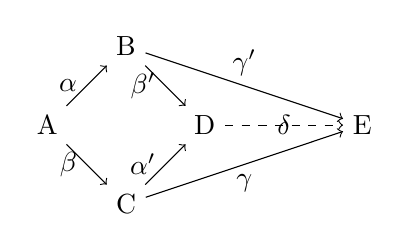
\begin{tikzpicture}
                \node (i) at (0,0) {A};
                \node (r) at (1,1) {B};
                \node (c) at (1,-1) {C};
                \node (h) at (2,0) {D};
                % \node () at (1,-1) {\( \Delta \)};
                \draw[->]  (i) -- (r) node [midway,left] {$ \alpha $};
                \draw[->] (c) -- (h) node [midway,left] {$ \alpha' $};
                \draw[->] (r) -- (h) node[midway, left] {$ \beta' $};
                \draw[->] (i) -- (c) node[midway, left] {$ \beta $};
                \node (d') at (4,0) {E};
                \draw[->] (c) -- (d') node [midway,below]{$ \gamma $};
                \draw[->] (r) -- (d') node [midway,above]{$ \gamma' $};
                \draw[->,dashed] (h) -- (d') node [midway]{$ \delta $};
            \end{tikzpicture}
}
\end{minipage}
The diagram involving \( (\alpha, \beta, \alpha', \beta') \) is called the \textbf{pushout square}, with \(D\) as the \textbf{pushout object}. The existence of a unique morphism is known as the universal mapping property of the pushout.
\end{definition} 
\begin{example}
    \label{ex:cat:po}
    Consider the square in \textbf{Graph} illustrated below.
    A pushout of the span \( B \overset{\alpha}{\leftarrowtail} A \overset{\beta}{\rightarrowtail} C \) is the cospan \( C \overset{\alpha'}{ 
    \rightarrowtail} D \overset{\beta'}{\leftarrowtail} B \), where pushout object \( D \) is the graph union of $B$ and $C$ and the morphisms \( \alpha' \) and \( \beta' \) are inclusion functions. 

    \begin{center} 
        \resizebox{0.45\textwidth}{!}{
        \begin{tikzpicture} 
            \graphbox{\( B \)}{40mm}{20mm}{34mm}{12mm}{2mm}{2mm}{
                \coordinate (o) at (0mm,-8mm); 
                \node[draw,circle] (l1) at ($(o)+(-10mm,0mm)$) {1};
                \node[draw,circle] (l2) at ($(l1)+(2,0)$) {2};
                \node[draw,circle,red] (l3) at ($(l1) + (1,0)$) {3};
                \draw[->,red] (l1) -- (l3) node[midway,above] {$a$};
                \draw[->,red] (l3) -- (l2) node[midway,above] {$a$};
            } 
    
            \graphbox{\( A \)}{0mm}{0mm}{34mm}{12mm}{2mm}{2mm}{
                \coordinate (o) at (0mm,-8mm); 
                \node[draw,circle] (l1) at ($(o)+(-10mm,0mm)$) {1};
                \node[draw,circle] (l2) at ($(l1)+(2,0)$) {2};
            }  
            \graphbox{\( D \)}{90mm}{5mm}{34mm}{22mm}{2mm}{-3mm}{
                \coordinate (o) at (0mm,-3mm); 
                \node[draw,circle] (l1) at ($(o)+(-10mm,0mm)$) {1};
                \node[draw,circle] (l2) at ($(l1)+(2,0)$) {2};
                \node[draw,circle,red] (l3) at ($(l1) + (1,0)$) {3};
                \node[draw,circle,blue] (l4) at ($(l2) + (0,-1)$) {6};
                \draw[->,red] (l1) -- (l3) node[midway,above] {$a$};
                \draw[->,red] (l3) -- (l2) node[midway,above] {$a$};
                \draw[->,blue] (l2) -- (l4) node[midway,right] {$a$};
                \node[draw,circle,blue] (l6) at ($(l1) + (0,-1)$) {7};
                \draw[<-,blue] (l1) -- (l6) node[midway,left] {$a$};
                \draw[->,blue] (l2) edge[out=-135,in=-45]node[midway,below] {$a$} (l1) ;
            }    
     
            \graphbox{\( C  \)}{40mm}{-20mm}{34mm}{22mm}{2mm}{-3mm}{
                \coordinate (o) at (0mm,-3mm); 
                \node[draw,circle] (l1) at ($(o)+(-10mm,0mm)$) {1};
                \node[draw,circle] (l2) at ($(l1)+(2,0)$) {2};
                \node[draw,circle,blue] (l4) at ($(l2) + (0,-1)$) {6};
                \draw[->,blue] (l2) -- (l4) node[midway,right] {$a$};
                \draw[->,blue] (l2) edge[out=-135,in=-45]node[midway,below] {$a$} (l1) ;
                \node[ draw,circle,blue] (l6) at ($(l1) + (0,-1)$) {7};
                \draw[<-,blue] (l1) -- (l6) node[midway,left] {$a$};
            }      
            % K to L
            \draw[>->] (17mm,5mm) -- node[above] {$\alpha$} (37mm,15mm);
            % C to G
            \draw[>->] (76mm,-28mm)-- node[below] {$\alpha'$} (104mm,-20mm) ;
            % K to C
            \draw[>->] (17mm,-17mm) -- node[below] {$\beta$} (37mm,-28mm);
            % L to G
            \draw[>->] (76mm,16mm) -- node[above] {$\beta'$} (104mm,7mm);
            \node () at (57mm,-6mm) {$PO$};
        \end{tikzpicture}
        }
    \end{center}
\end{example}
\begin{definition}[Pullback \cite{pierce1991basic}]
    \label{def:cat:pb}
    \ \newline
\noindent
\begin{minipage}{0.7\textwidth}  
   A \textbf{pullback} of a cospan \(B \overset{\beta'}{\rightarrow} D \overset{\alpha'}{\leftarrow} C \), as shown on the right, is defined as a span \( B \overset{\alpha}{\leftarrow} A \overset{\beta}{\rightarrow} C \) such that \( \alpha \star \beta' = \beta \star \alpha' \), and for every span \( B \overset{\gamma'}{\leftarrow} E \overset{\gamma}{\rightarrow} C \) if \(\gamma' \star \beta' = \gamma \star \alpha'\) holds, then there exists a unique morphism \(\delta: E \to A\) such that $\gamma' = \delta \star \alpha$ and $\gamma = \delta \star \beta$. 
\end{minipage}
\hfill
\begin{minipage}{0.299\textwidth}
    \hfill
\resizebox{0.9\textwidth}{!}{
            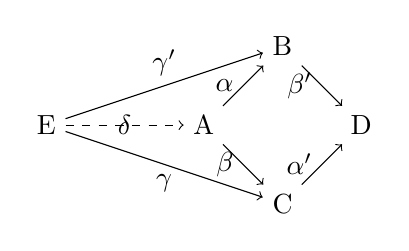
\begin{tikzpicture}
                \node (i) at (0,0) {A};
                \node (r) at (1,1) {B};
                \node (c) at (1,-1) {C};
                \node (h) at (2,0) {D};
                % \node () at (1,-1) {\( \Delta \)};
                \draw[->]  (i) -- (r) node [midway,left] {$\alpha$};
                \draw[->] (c) -- (h) node [midway,left] {$\alpha'$};
                \draw[->] (r) -- (h) node[midway, left] {$\beta'$};
                \draw[->] (i) -- (c) node[midway, left] {$\beta$};
                \node (d') at (-2,0) {E};
                \draw[<-] (c) -- (d') node [midway,below]{$\gamma$};
                \draw[<-] (r) -- (d') node [midway,above]{$\gamma'$};
                \draw[->, dashed] (d') -- (i) node [midway]{$\delta$};
            \end{tikzpicture}
}
\end{minipage}
The diagram involving \( (\alpha, \beta, \alpha', \beta') \) is called the \textbf{pullback square}, with \(A\) as the \textbf{pullback object}. The existence of a unique morphism is known as the universal mapping property of the pullback.
\end{definition} 
 
\begin{definition}
    \label{def:cat:pb}
    Consider the square in \autoref{ex:cat:po}. A pullback of the cospan \( C \overset{\alpha'}{\rightarrowtail} D \overset{\beta'}{\leftarrowtail} B \) is the span \( B \overset{\alpha}{\leftarrowtail} A \overset{\beta}{\rightarrowtail} C \), where pullback object \( A \) is the graph intersection of $B$ and $C$ and the morphisms \( \alpha \) and \( \beta \) are inclusion functions.
\end{definition}
\begin{notation}
    When the context makes it clear, a morphism \( h : A \to B \) will be denoted by \( h_{AB} \), and diagrams will be referred to by their nodes, as is standard in geometry. For example, the diagram involving morphisms \( ( \alpha, \beta, \alpha', \beta' ) \) in \autoref{def:cat:po} will be denoted by \( ACDB \) or \( ABDC \).
\end{notation}   